\documentclass[11pt,a4paper,USenglish]{article}
\usepackage{ttk4135LabReport}

\usepackage{babel}
\usepackage{amsmath,amssymb}
\usepackage[utf8]{inputenc}
\usepackage{graphicx}
\usepackage{epstopdf}
\usepackage[round]{natbib}
\usepackage{tocbibind}
\usepackage[thinspace,amssymb]{SIunits}
\usepackage{listings, courier, color}
\usepackage[margin=2.5cm]{geometry}
\usepackage{libertine}
\usepackage{fancyref}
\usepackage{newtxmath}
\usepackage{afterpage}
\usepackage[T1]{fontenc}
\graphicspath{{../}}
\lstset{inputpath={../}}
\usepackage[hidelinks]{hyperref} % Always load last

\studentnumbers{736698, 742388, 742367, 755875 and 731918}
\groupnumber{17}
\date{May 1, 2015}

\begin{document} 
 
\makelabreportfrontpage
\begin{abstract}\addcontentsline{toc}{section}{Abstract}
This document outlines a few important aspects of the lab report. It contains some advice on both content and layout. The Latex source for this document is also published, and you can use it as a template of sorts for your own report.

When you write your own report, this section (the abstract) should contain a \emph{very} short summary of what the lab is about and what you have done.
\end{abstract} 
\tableofcontents
\section{Intro}
\subsection{Modeling, linearization}
On this project we will be using optimization theory to control a model of a helicopter. This is done by:
 making a non-linear model of the helicopter, and the linearize it at an equilibrium. This method is widely used in control theory and works well if the system operates near or at the equilibrium or have quite small non-linearities. However when this is not the case, a linearized model may not be adequate for stabilizing and controlling the system.

 The reason most control engineers prefer linear model is the ability to analyze them and tune regulators. In this project we linearize one time manually around an equilibrium, but there is no limitations on the number of times the model can be linearized and the process can be done automatically by a computer. More about this in the last section.

\subsection{Optimal control, limitations without feedback}
Optimization theory is a knowledge used in many applications, from economy and production planing to control theory. In this project we will be looking at the last application, and how it can be used to solve control theory problems. The main difference between a conventional regulator who only uses the current state or output and a reference and a trajectory from an optimization over a horizon is the ability to "look into the future". 

While a conventional regulator will calculate an error and correct the input thereafter, a planned trajectory from an optimization problem will contain inputs for the complete horizon. However, there can be quite drastic drawbacks with implementing this optimal sequence of inputs directly to the system since there are no feedback, any error caused by modeling errors and disturbances will accumulate and often cause drift and maybe instability.

\subsection{Optimal control, trust the trajectory not the input}
However, while the optimal sequence of inputs may not be perfect in open-loop, the planned trajectory for the states are often quite useful, even if the model have errors. Here it is possible to implement a traditional PID regulator, or as we will be doing in this project, implement a linear quadratic regulator (LQR). 

The LQR can be both time variant and time invariant, dictated by the nature of the system. As mentioned in the linearizion part, the calculation of the LQR gain can and will be done by a computer, and will often be recalculated when re-linearizing. By tuning the LQR so that it prioritize to follow the trajectory of the states rather than following the optimal input, it is possible to compensate for modeling errors.

\subsection{Optimal control with non-linear constraints, and thoughts on MPC}
When controlling two degrees of freedom with non-linear inequality constraints with optimization theory, the time it takes to solve the optimization problem is quite long. When calculating the trajectory once and then executing the whole horizon this does not become a problem.

However when using MPC, which is to recalculate the horizon every time step and only use the first calculated input, this time becomes a problem. This calculation time can be improved by selecting a better solver, increase hardware specifications and do simplifications / linearizion. When achieving this on a low-power unit like a micro controller, FPGA, DSP or equivalent, a new world in control theory will open.

\section{Problem Description}\label{sec:prob_descr}

\subsection{Hardware setup}
The helicopter is fixed to a base and has an extended arm with motors attached at one end,
and a balance weight at the other. We parametrize the helicopter state by three rotations:
\begin{itemize}
    \item Travel ($\lambda$): At the base about the vertical axis
    \item Elevation ($e$): At the arm joint about a horizontal axis
    \item Pitch ($p$): At the head joint about the arm axis
\end{itemize}
These angles are measured by the encoders at each rotational joint. We can affect the motion by adjusting the voltage input to the DC motors. Propellers are attached to the motors, and the thrust generated is assumed to be proportional to the voltage applied, with identical motor constant for both motors. Figure (\ref{fig:hardware}) shows the helicopter and the relevant angles. Table (\ref{tab:parameters}) shows the parameters for the helicopter used in the report.

\begin{figure}[htb]
	\centering
	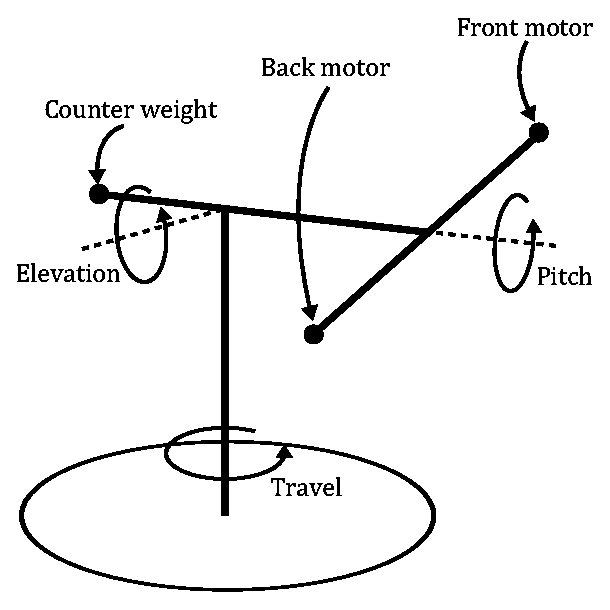
\includegraphics[width = 0.55\textwidth]{figures/hardware_setup.eps}
	\caption{The helicopter hardware setup}
	\label{fig:hardware}
\end{figure}

\subsection{Software setup}
We use Simulink and Matlab to implement the control program, and interface with the helicopter through QuaRC and Realtime Workshop. See [\cite{LabExercise}] for more information.

\subsection{Model discussion}
In order to compute an optimal control input, we need some measure of optimality.
To this extent, we use a discrete-time state-space model, that describes the motion
of our helicopter given an input sequence. The first step is to derive the equations
of motions in continuous-time. We do this by considering torque balances about each
rotation axis, and applying Newton's law. A full derivation is not interesting, so
we refer to the exercise text [\cite{LabExercise}] and list the resulting set of
differential equations below.
\begin{subequations}
\label{eq:model_al}
\begin{align}
    \ddot{e} + K_{3} K_{ed} \dot{e} + K_{3} K_{ep} e &= K_{3} K_{ep} e_{c} \label{eq:model_se_al_elev} \\
    \ddot{p} + K_{1} K_{pd} \dot{p} + K_{1} K_{pp} p &= K_{1} K_{pp} p_{c} \label{eq:model_se_al_pitch} \\
    \dot{\lambda} &= r \label{eq:model_se_al_lambda} \\
    \dot{r} &= -K_{2} p \label{eq:model_se_al_r}
\end{align}
\end{subequations}

The associated nomenclature is listed in table (\ref{tab:variables}). This model deserves some discussion. First, a complete model would have (non-linear) trigonometric terms. But such a model is impractical for use in dynamic optimization schemes. Instead, we linearize the model by assuming that the pitch and elevation angles are both very close to zero.

The resulting model has the advantage of being compatible with highly efficient techniques that have been developed specifically for linear optimization problems. It is however a very simple model, and omits any interaction between elevation and pitch angle/travel. While there will always be modelling errors due to process noise, or inaccurate measurements/parameters, this simplification will affect the computed optimal control. We can dampen the effect from the error by keeping the system close to the linearization point, for instance by constraining the angles to be within a margin around equilibrium.

Second, the model incorporates a PID controller for the elevation, which is assumed to counteract the constant torque due to gravity, as well as a PD controller for the pitch. The result of this is that our goal in the optimization problem is to compute the setpoints, $e_c$ and $p_c$. Computing the appropriate voltages is left to the internal controllers.

\begin{table}[ht]
    \centering
    \caption{Parameters and values}
    \begin{tabular}{llll}
        \hline
        Symbol & Parameter & Value & Unit \\
        \hline
        $l_a$ & Distance from elevation axis to helicopter body & $0.63$ & \meter \\
        $l_h$ & Distance from pitch axis to motor & $0.18$ & \meter \\
        $K_f$ & Force constant motor & $0.20$ & \newton\per\volt \\
        $J_e$ & Moment of inertia for elevation & $1.11$ & \kilogram\usk\square\meter \\
        $J_t$ & Moment of inertia for travel & $1.11$ & \kilogram\usk\square\meter \\
        $J_p$ & Moment of inertia for pitch & $0.045$ & \kilogram\usk\square\meter \\
        $m_h$ & Mass of helicopter & $1.42$ & \kilogram \\
        $m_w$ & Balance weight & $1.80$ & \kilogram \\
        $m_g$ & Effective mass of the helicopter & $0.025$ & \kilogram \\
        $K_p$ & Force to lift the helicopter from the ground & $0.25$ & \newton \\
        \hline
    \end{tabular}
    \label{tab:parameters}
\end{table}

\begin{table}[ht]
    \centering
    \caption{Variables}
    \begin{tabular}{ll}
    \hline
    Symbol & Variable \\
    \hline
    $p$                    & Pitch \\
    $p_c$                  & Setpoint for pitch \\
    $\lambda$              & Travel \\
    $r$                    & Speed of travel \\
    $r_c$                  & Setpoint for speed of travel \\
    $e$                    & Elevation \\
    $e_c$                  & Setpoint for elevation \\
    $V_f$                  & Voltage, motor in front \\
    $V_b$                  & Voltage, motor in back \\
    $V_d$                  & Voltage difference, $V_f - V_b$ \\
    $V_s$                  & Voltage sum, $V_f + V_b$ \\
    $K_{pp},K_{pd},K_{ep},K_{ei}, K_{ed}$ & Controller gains \\
    $T_g$                  & Moment needed to keep the helicopter flying \\
    % $\lambda^*$
    % $e_c^*$
    \hline
    \end{tabular}
    \label{tab:variables}

TODO: Variable notation for plots and stuff.
\end{table}

\section{Repetition/Introduction to Simulink/QuaRC}\label{sec:prob1}

This part is just a repetition, and therefore does not contain any important results. However, the part is important because it is used to test the hardware setup at the lab. This was done using a handed out script that made the helicopter hover at zero elevation and zero pitch. The helicopter suffered from minor drifting as a result of not perfectly tuned motor constants in the handed out script. This was expected and does not really introduce any problem since the drifting would be eliminated as soon as some form of feedback was implemented.
\section{Optimal Control of Pitch and Travel without Feedback}\label{sec:prob2}

In this section we compute an optimal trajectory $x^*$ and a corresponding input sequence $u^*$. The trajectory should bring the helicopter from an initial state to another predefined state. We do not use feedback to correct for deviations from the calculated trajectory. Furthermore, we disregard elevation, that is, we assume $e=0$. The computation of the optimal trajectory was formulated as a convex optimization problem.

\subsection{The helicopter model on continuous-time state-space form}

The system (\ref{eq:model_al}) describes the helicopter plant, with a basic control layer consisting of PID and PD controllers for elevation and pitch. The optimization layer gives the inputs to these regulators, as shown in figure (\ref{fig:control_hierarchy}).

\begin{figure}[ht]
	\centering
	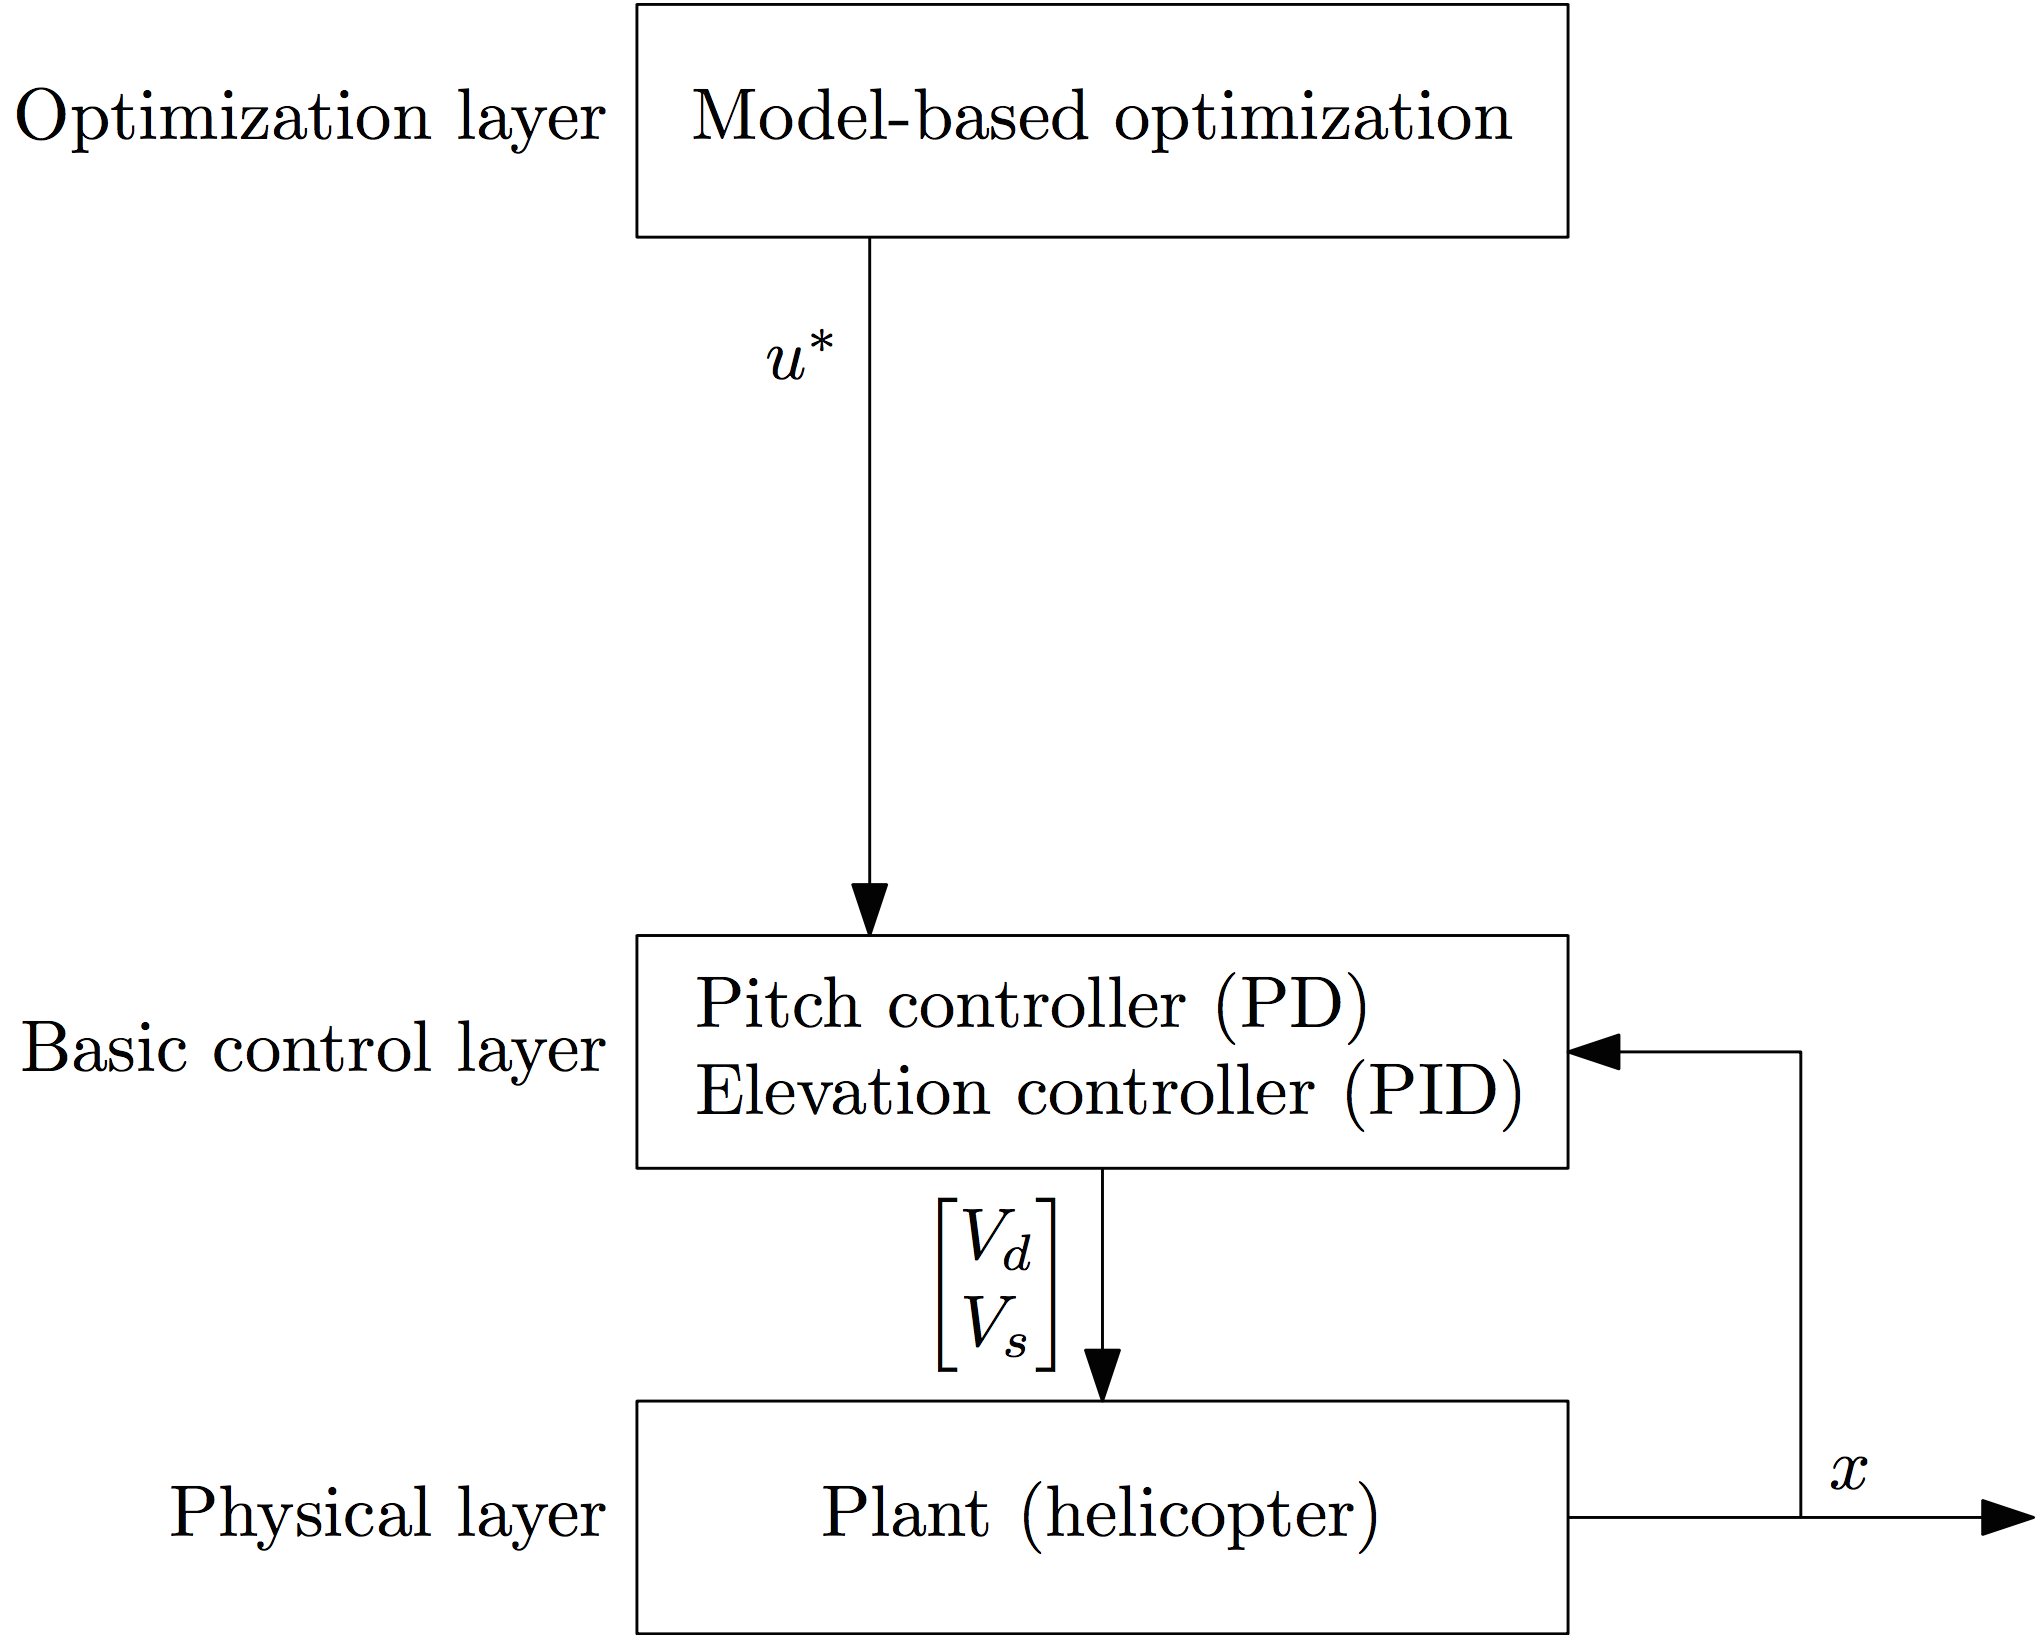
\includegraphics[width=0.6\textwidth]{figures/day2/control_hierarchy_day2}
	\caption{Control hierarchy}
	\label{fig:control_hierarchy}
\end{figure}

The system can be written on continuous-time state-space form:

\begin{equation}
    \dot{x} = A_cx + B_cu
    \label{eq:state_space_axbu}
\end{equation}

with $x = \begin{bmatrix} \lambda & r & p & \dot{p} \end{bmatrix}^T$ and $u = p_c$.
The continuous-time system matrices for this model are:

\begin{equation}
	A_c = \begin{bmatrix} 0 & 1 & 0 & 0 \\ 0 & 0 & -K_2 & 0 \\ 0 & 0 & 0 & 1 \\ 0 & 0 & -K_1K_{pp} & -K_1K_{pd} \end{bmatrix}
	\qquad\text{and}\qquad
	B_c = \begin{bmatrix}0 \\ 0 \\ 0 \\K_1K_{pp} \end{bmatrix}
\end{equation}


\subsection{Discretization}

The system dynamics was implemented as a sequence of constraints in the optimization problem, and the system model therefore had to be written in discrete-time state-space form,

\begin{equation}
	x_{k+1} = Ax_k + Bu_k.
	\label{eq:discrete_state_space_axbu}
\end{equation}

The model was discretized using the Forward-Euler method with timestep $h$.

\begin{equation}
	\dot{x}_k \approx \frac{x_{k+1} - x_k}{h}
\end{equation}

Inserting this into (\ref{eq:state_space_axbu}),

\begin{equation}
	\dot{x}_{k+1} \approx (I + hA_c) x_k + hB_c u_k
\end{equation}

is obtained. A suitable approximation for the discrete-time matrices is then

\begin{equation}
	A \approx I + hA_c
	\qquad\text{and}\qquad
	B \approx hB_c
\end{equation}

These matrices were computed in Matlab, and are therefore not shown explicitly here.


\subsection{Computation of optimal trajectory}

An optimal trajectory can be generated by minimizing the cost function

\begin{equation}
	\label{eq:trajectory_cost}
	\phi = \sum_{i=1}^{N}(\lambda_i - \lambda_f)^2 + qp_{ci}^2
\end{equation}

for some scalar weight $q \geq 0$ over the finite horizon of states and inputs

\begin{equation}
	z = (x_1 \; x_2 \; ... \; x_N \; u_1 \; u_2 \; ... \; u_N)^T
\end{equation}

This was done in Matlab using the function quadprog. The discrete system dynamics was implemented as equality constraints of the form $A_{\text{eq}}z = B_{\text{eq}}$, where $A_{\text{eq}}$ and $B_{\text{eq}}$ are given by the left- and right-hand side of the $N$ constraints

\begin{align*}
	x_1 - Bu_0        &= Ax_0 \\
	x_2 - Ax_1 - Bu_1 &= 0    \\
	\vdots                    \\
	x_N - Ax_{N-1} - Bu_{N-1} &= 0
\end{align*}

We would also like to constrain the system state and input to be within a range

\begin{align}
	x^{\text{min}} \leq x_{t+1} \leq x^{\text{max}} \\
	u^{\text{min}} \leq u_t \leq u^{\text{max}}
\end{align}

for $t = 0...N-1$. Applying these constraints to all states and inputs in the solution horizon, we have

\begin{equation}
	\begin{bmatrix} I \\ -I \end{bmatrix} z
	\leq
	\begin{bmatrix}
	\{x_{t+1}^{max}\} \\
	\{u_t^{max}\} \\
	\{x_{t+1}^{min}\} \\
	\{u_t^{min}\}
	\end{bmatrix}_{t=0..N-1}
\end{equation},

which can be implemented as an inequality constraint of the form $A_{\text{iq}} z \leq B_{\text{iq}}$. Solving the optimization problem with different weights $q$ did not lead to any significant differences in the trajectory, this because the model inaccuracies made the helicopter drift away from the desired state anyway.

The objective function (\ref{eq:trajectory_cost}) weights %er dette riktig ord for å vekte noe?
the input relative to the state deviations using the weight parameter $q$. The term $(\lambda_i - \lambda_f)^2$ is the state deviations. They are squared to prioritize the largest deviation. Note that the cost function (\ref{eq:trajectory_cost}) does not take into consideration that $\lambda_i$ plus some multiple of $2\pi$ describes the same physical orientation of the helicopter. For example, if the reference is $0$ and $\lambda_i = 2\pi$, it will be regarded as a large error, even though the helicopter is in fact in the desired orientation. A more optimal scheme would take this into consideration.


\subsection{Implementation}

Figure (\ref{fig:day2_plot}) shows the implementation with $q = 1$. Zeroes were added on both sides of the input sequence to give time to initialize and stabilize the helicopter. As can be seen from the figure, the helicopter does not reach its desired final state.

\begin{figure}[htb]
	\centering
   		\makebox[\textwidth][c]{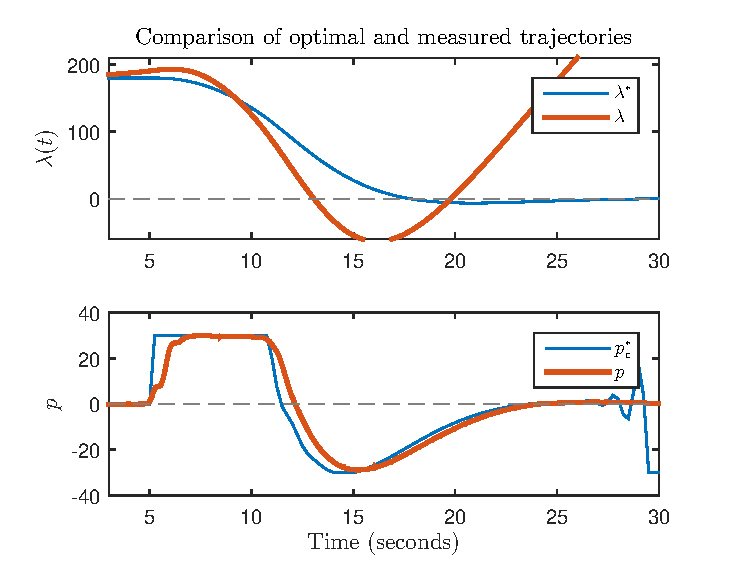
\includegraphics[width=\textwidth]{figures/day2/plot_day2}}
	\caption{Plot of day 2}
	\label{fig:day2_plot}
\end{figure}

The deviation was caused by an imperfect model. A perfect model is  unrealistic to construct, and without feedback, the model inaccuracies will lead to nonoptimal results in the real world. For example, the pitch-regulator in our model is fast enough to follow its input perfectly, and we are using a linear model that clearly does not correspond perfectly to the real helicopter.

\section{Optimal Control of Pitch/Travel with Feedback (LQ)}\label{sec:prob3}
This problem involves implementing an LQ controller for optimal control with feedback. We will calculate a gain matrix K using the LQ controller, implement feedback on the helicopter, and look into if MPC is a good alternative to LQ.

\subsection{Calculating the gain matrix K}
For calculating the gain matrix K we needed to use the matlab function dlqr, which is a linear-quadratic regulator design that minimiizes the cost function:
\begin{equation}
J = Sum {x'Qx + u'Ru + 2*x'Nu}
\end{equation}.
This function depend on the system matrices A and B aswell as Q and R, which we will need to choose an appropriate weight on. At first we choose Q and R as:

\begin{equation}
\mathbf{Q} =
\begin{bmatrix}
1 & 0 & 0 & 0 \\
0 & 1 & 0 & 0 \\
0 & 0 & 1 & 0 \\
0 & 0 & 0 & 1
\end{bmatrix}
\qquad\bold{R}=
\begin{bmatrix}
1
\end{bmatrix}
\end{equation}

 By trial and error we got the best result by penalizing the state for travel a lot more than the pitch. This gave us a new Q matrix on the form:

\begin{equation}
\mathbf{Q} =
\begin{bmatrix}
50 & 0 & 0 & 0 \\
0 & 1 & 0 & 0 \\
0 & 0 & 1 & 0 \\
0 & 0 & 0 & 1
\end{bmatrix}
\end{equation}

\subsection{Implementing feedback on the helicopter}
An implementation of feedback can be seen on the simulink diagram.

%Figure of simulink model with feedback
\begin{figure}[htb]
	\centering
   	 \makebox[\textwidth][c]{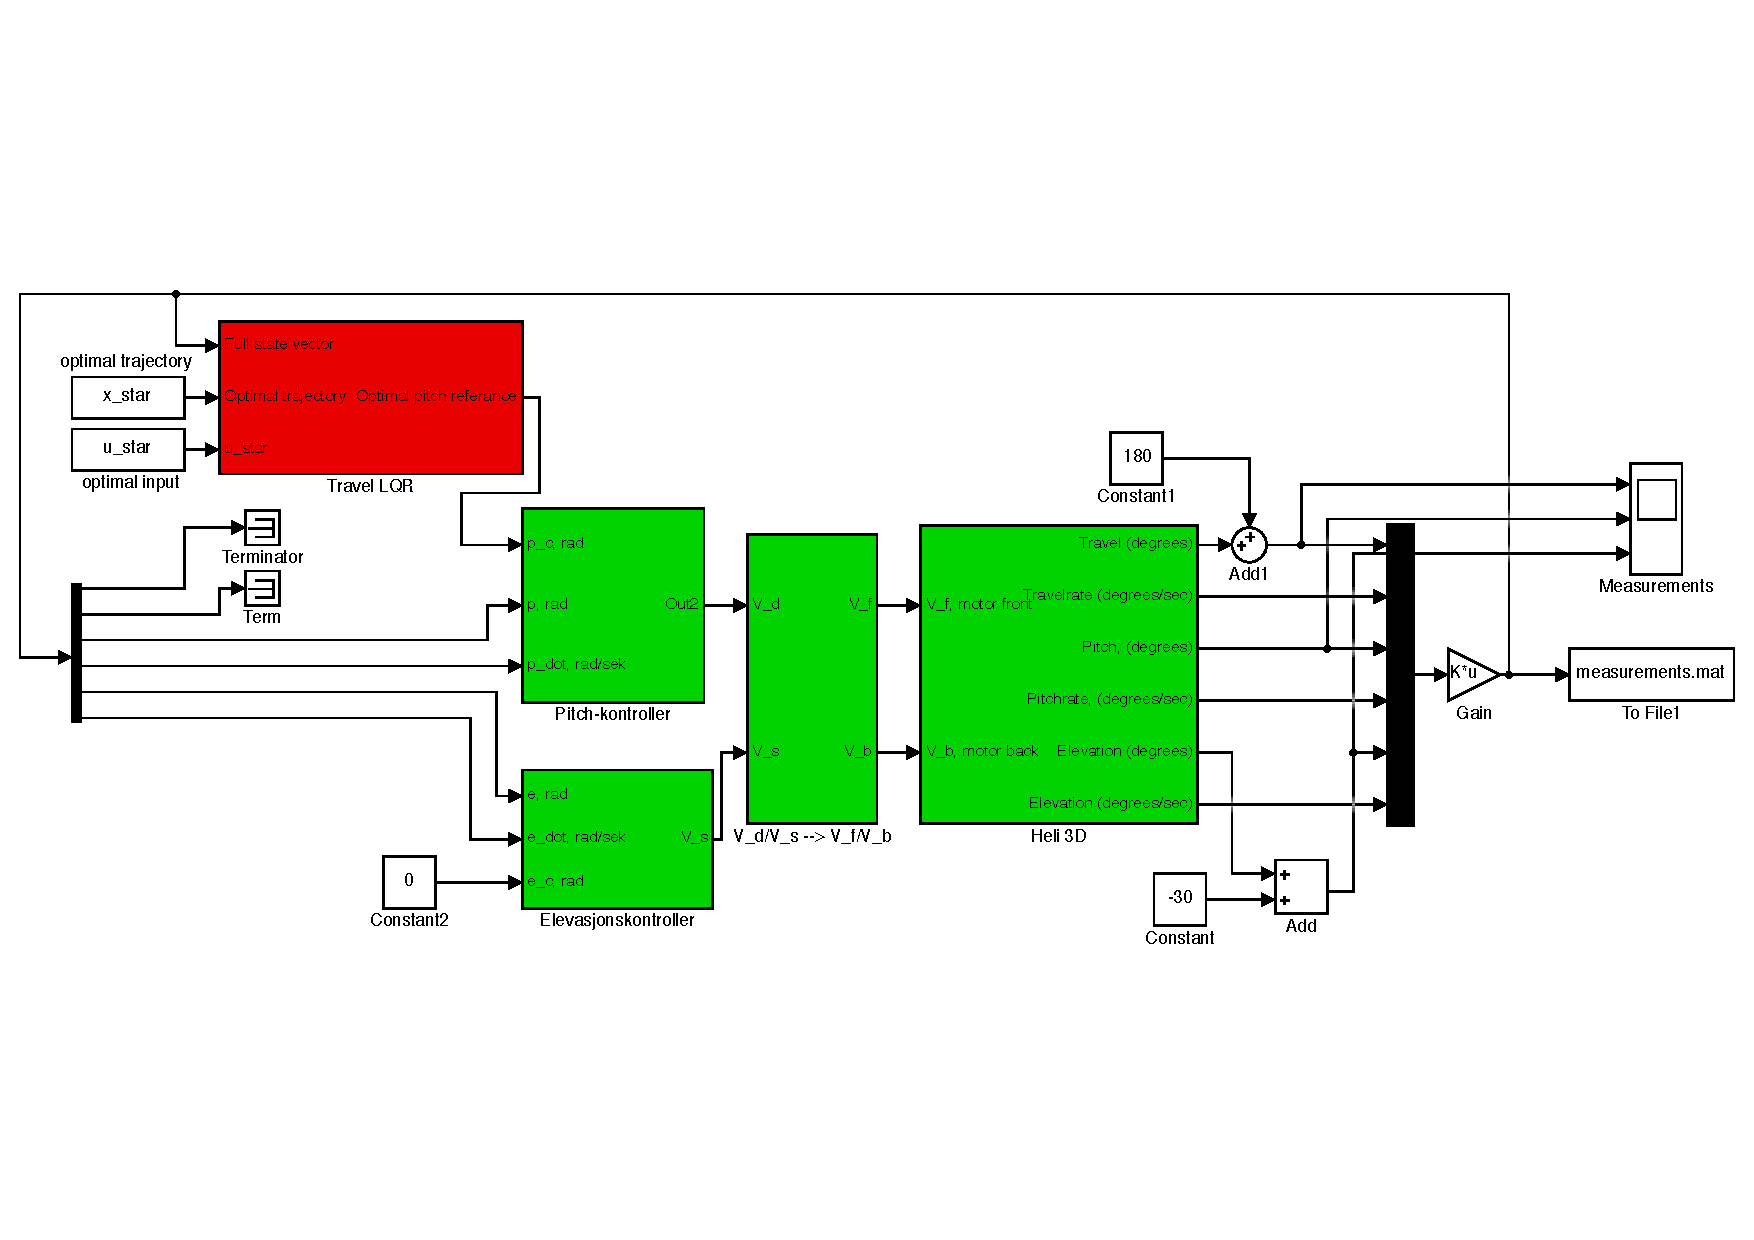
\includegraphics[width=1.2\textwidth]{figures/day3/day3_mdl}}
	\caption{Simulink model with feedback}
	\label{fig:day3_mdl}
\end{figure}

By using the gain matrix K calculated in last task, we see that by penalizing travel hard and pitch soft, the helicopter follows the travel trajectory closer than when weighting all states the same.
%Figure of helicopter response for Q_LQR = diag[50 1 1 1]
\begin{figure}[htb]
	\centering
    	\makebox[\textwidth][c]{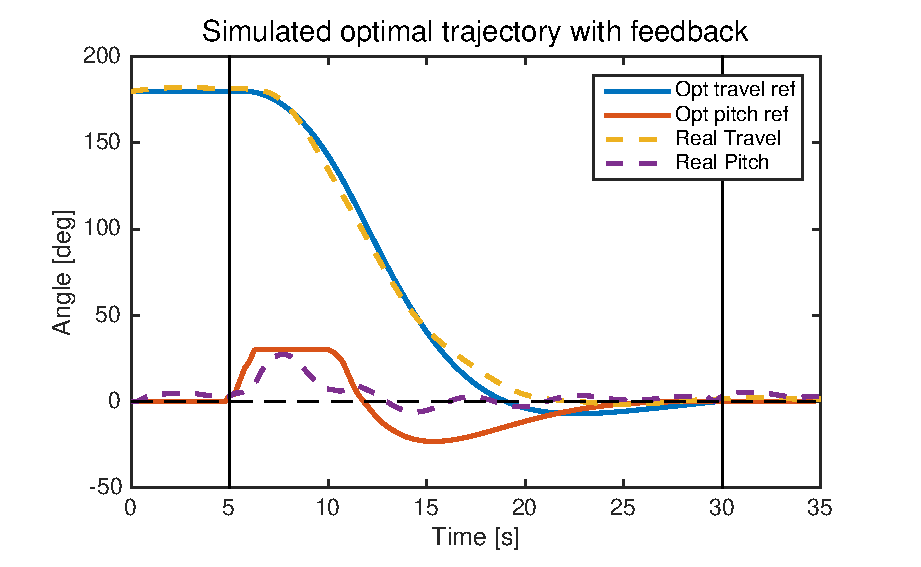
\includegraphics[width=1.2\textwidth]{figures/day3/plot_day3_q_50_1_1_1}}
	\caption{Plot of day 3 with Q = diag(50 1 1 1 )}
	\label{fig:day3_plot_50_1_1_1}
\end{figure}

We also tried penalizing the pitch more than travel, which gave us a bad result. This because the optimal pitch reference trajectory is based on a bad model.
%Figure of helicopter response for Q_LQR = diag[1 1 10 1]
\begin{figure}[htb]
	\centering
    	\makebox[\textwidth][c]{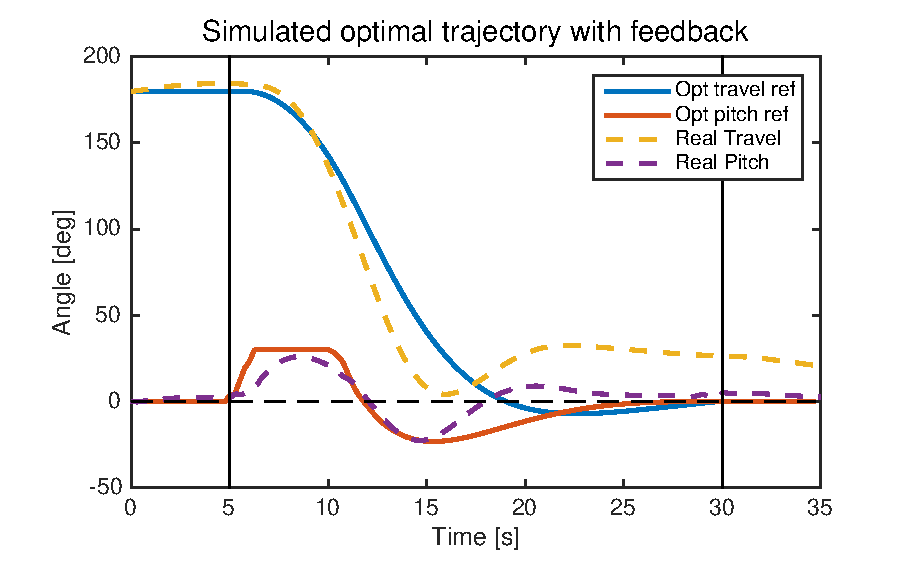
\includegraphics[width=1.2\textwidth]{figures/day3/plot_day3_q_1_1_10_1}}
	\caption{Plot of day 3 with Q = diag(1 1 10 1 )}
	\label{fig:day3_plot_1_1_10_1}
\end{figure}

\subsection{Comparison between LQR and MPC}
The way to implement an MPC controller would be to use the same procedure as for the LQR, but for every time step. Then using the first time step as the input u.

The advantages of using MPC instead of LQR; is that it gives us the possibility to have constraints in the regulator, can potentially produce a trajectory which performs its' task more cheaper and we get a implicit feedback with the use of MPC.
The main disadvantage of using MPC is that the calculations are a lot heavier to perform.
%Figure of figure 8, but with MPC implemented instead (if we have a figure of this)

\section{Optimal Control of Pitch/Travel and Elevation with and without Feedback}\label{sec:prob4}
In this section we extend our model to include the remaining states: elevation, $e$, and elevation
rate, $\dot{e}$. We use a non-linear solver to compute an optimal trajectory in two dimensions,
and additionally constrain the elevation to avoid a restriction shaped as a bell-curve.

\subsection{State-space formulation}
The state-vector is extended with the remaining states, 
\begin{subequations}
\label{eq:day4_cost}
    x = \begin{bmatrix} \lambda & r & p & \dot{p} & e & \dot{e} \end{bmatrix}^T, 
\end{equation}
and the input-vector also contains the elevation setpoint fed to the internal controller, 
\begin{equation}
    u = \begin{bmatrix} p_c & e_c \end{bmatrix}^T.
\end{equation}
The system is on the usual state-space form (\ref{eq:state_space_axbu}),
with
\begin{equation}
    \dot{x} =
    \underbrace{
    \begin{bmatrix}
    0 & 1 &      0     &      0     &      0     &      0    \\
    0 & 0 &    -K_2    &      0     &      0     &      0    \\
    0 & 0 &      0     &      1     &      0     &      0    \\
    0 & 0 & -K_1K_{pp} & -K_1K_{pd} &      0     &      0    \\
    0 & 0 &      0     &      0     &      0     &      1    \\
    0 & 0 &      0     &      0     & -K_3K_{ep} & -K_3K_{ed}
    \end{bmatrix}}_{A_c}
    x +
    \underbrace{
    \begin{bmatrix}
        0       &     0     \\
        0       &     0     \\
        0       &     0     \\
    K_1K_{pp}   &     0     \\
        0       &     0     \\
        0       & K_3K_{ep}
    \end{bmatrix}}_{B_c}
    u
    \label{eq:extended_state_space}
\end{equation}

\subsection{Discretization}
We discretize (\ref{eq:extended_state_space}) using the same method
as in section (\ref{sec:prob2}). That is, an approximation of the
discrete-time state-space matrices is
\begin{equation}
    A \approx I + hA_c
    \qquad\text{and}\qquad
    B \approx hB_c
\end{equation}
where $I$ is now the $6\times6$ identity matrix.

\subsection{Modelling the restriction}
A common application of optimal control is to implement restrictions,
such as avoiding physical objects, as constraints in the optimization
problem. Such restrictions can not be enforced when using only state-
feedback controllers.

We wish to restrict the helicopter head to move above a bell-shaped curve
\begin{equation}
    e_k \geq \alpha \exp (-\beta (\lambda_k - \lambda_t)^2 )
\end{equation}
for all timesteps $k$ over the solution horizon. Since this is a non-linear constraint, we can no longer use a QP solver. Instead, a non-linear solver is needed, and in this case, the MATLAB function fmincon was used with a SQP-type algorithm.

% \section{Notater for dagen: 16. mars} % Fikk fmincon til å fungere, med ikke-lineær constraint. % TODO: Test uten LQR. Lag egen slx hvor vi kopler ut LQR blokka.
% TODO: Kjør tuning tester. Juster Q_LQR.

\subsection{Objective function}
For this assignment, the cost function was the same as in equation (\ref{eq:trajectory_cost}), but with an extra term for penalizing elevation. We chose to set up the cost function on a more general form:
\begin{equation}
    \phi=\sum(x^{T}Q_{LQR}x+u^{T}R_{LQR}u)
    
\end{equation}
Here, $Q_{LQR}$ and $R_{LQR}$ are diagonal matrices, with unity weight on $q_{travel}$, $r_{pitch}$ and $r_{elevation}$, so that it corresponds with the extended state and input vectors (\ref{eq:day4_cost}). %denne ligningen?

%This formulation makes it possible to easily put some weight on the other states as well, if deviation in these states should be penalized.

\subsection{Results}

For controlling the helicopter, we ended on a horizon of $N=60$ timesteps, or 15 seconds. This gave us an optimal trajectory that looked much the same as for assignment 3 for pitch and travel. In addition, an elevator trajectory just touching the top of the bell curve constraint was also calculated. The suggested horizon of $N=40$ did not terminate in reasonable time, and was therefore replaced by a longer horizon giving reasonable results.%forslag til bedre formulering?

The solution without feedback acted in the same manner as it did in section (\ref{sec:prob2}). As can be seen in figure (??) !!!!!, the real trajectory of travel and elevation tried to follow the optimal solution, but the effect of not having a perfect model becomes more and more clear as time passes, and at the end of the horizon, the travel drifted away from the solution just like in section (\ref{sec:prob2}).

Using state feedback LQR, the helicopter managed to follow the calculated trajectory quite good after some tuning. As in section (\ref{sec:prob3}), it was appropriate to weight deviation(s) in travel (and here also elevation) more than deviation in pitch. When the regulator is working on an inaccurate model, it is for the task given more constructive to try to follow the travel and elevation trajectories rather than the ideal, linearized input trajectory. This input will, given the unlinearities of the model, not lead to an appropriate response for the trajectories. The result, with different weights on the states of $Q_{LQR}$ can be seen in the following figures. %legge inn typ 3 figurer her med den beste og 2-3dårligere responser og i tillegg skrive på hva de ulike vektene er.

One thing worth noticing is that the trajectory of elevation consequently falls below the constraint at the peak of the constraint. We believe this is due to the fact that our model suggests that there is no link between the model for elevation, and that of pitch. They are in fact linked, and because of this, the regulator doesn't manage to meet both demands perfectly at the same time, and we get a deviation. If the model would include this crossing terms, the result would probably be better. The problem with this approach is that it leads to a non linear objective function, which takes longer time to compute for the solver.
% TODO: Add figure showing the helicopter following the non-linear constraint. Showing the associated input. Explain why the input looks like it does.
\begin{figure}[htb]
	\centering
   	 \makebox[\textwidth][c]{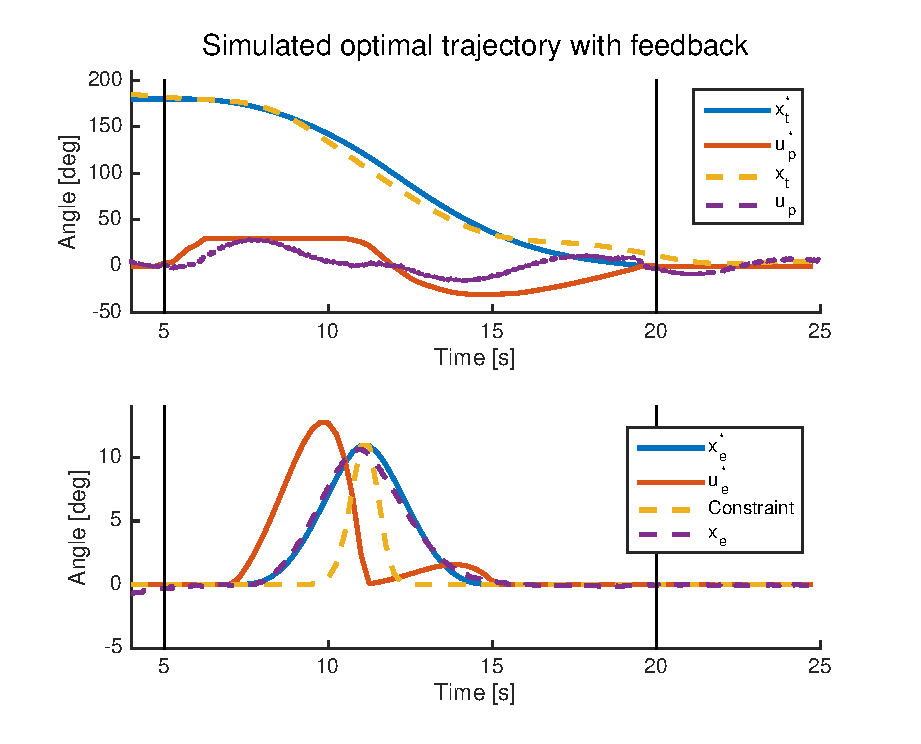
\includegraphics[width=1.2\textwidth]{figures/day4_cl/plot_day4_CL_q_20_1_1_1_30_10}}
	\caption{Plot day 4 closed loop Q=diag(20 1 1 1 30 10)}
	\label{fig:day4_cl_plot_20_1_1_1_30_10}
\end{figure}

% Notation:
% x_e^*: Computed elevation trajectory
% x_t^*: Computed travel trajectory
% u_p^*: Computed pitch setpoint sequence
% u_e^*: Computed elevation setpoint sequence


% Notat
% Cirka 11 sek ut i simuleringa, så ser vi at det er avvik mellom humpen og faktisk elevation, samtidig som det er avvik mellom travel-bane og faktisk travel. Vi har forsøkt å tune slik at elevation følger humpen tettere, men uten hell.

% Grunnen til dette tror vi er fordi det er en tradeoff i virkeligheten mellom å følge travel-banen og humpen. For å følge humpen bedre, så brukes pitch på en slik måte at det blir større avvik fra travel-banen. I modellen antas at pitch og elevation er fullstendig separerte, og dette problemet skal i teorien ikke oppstå. Men i virkeligheten er det en kobling.

% TODO: Forklar dette fenomenet. Referér til figuren, ved hump-toppen.
\begin{figure}[htb]
	\centering
   	 \makebox[\textwidth][c]{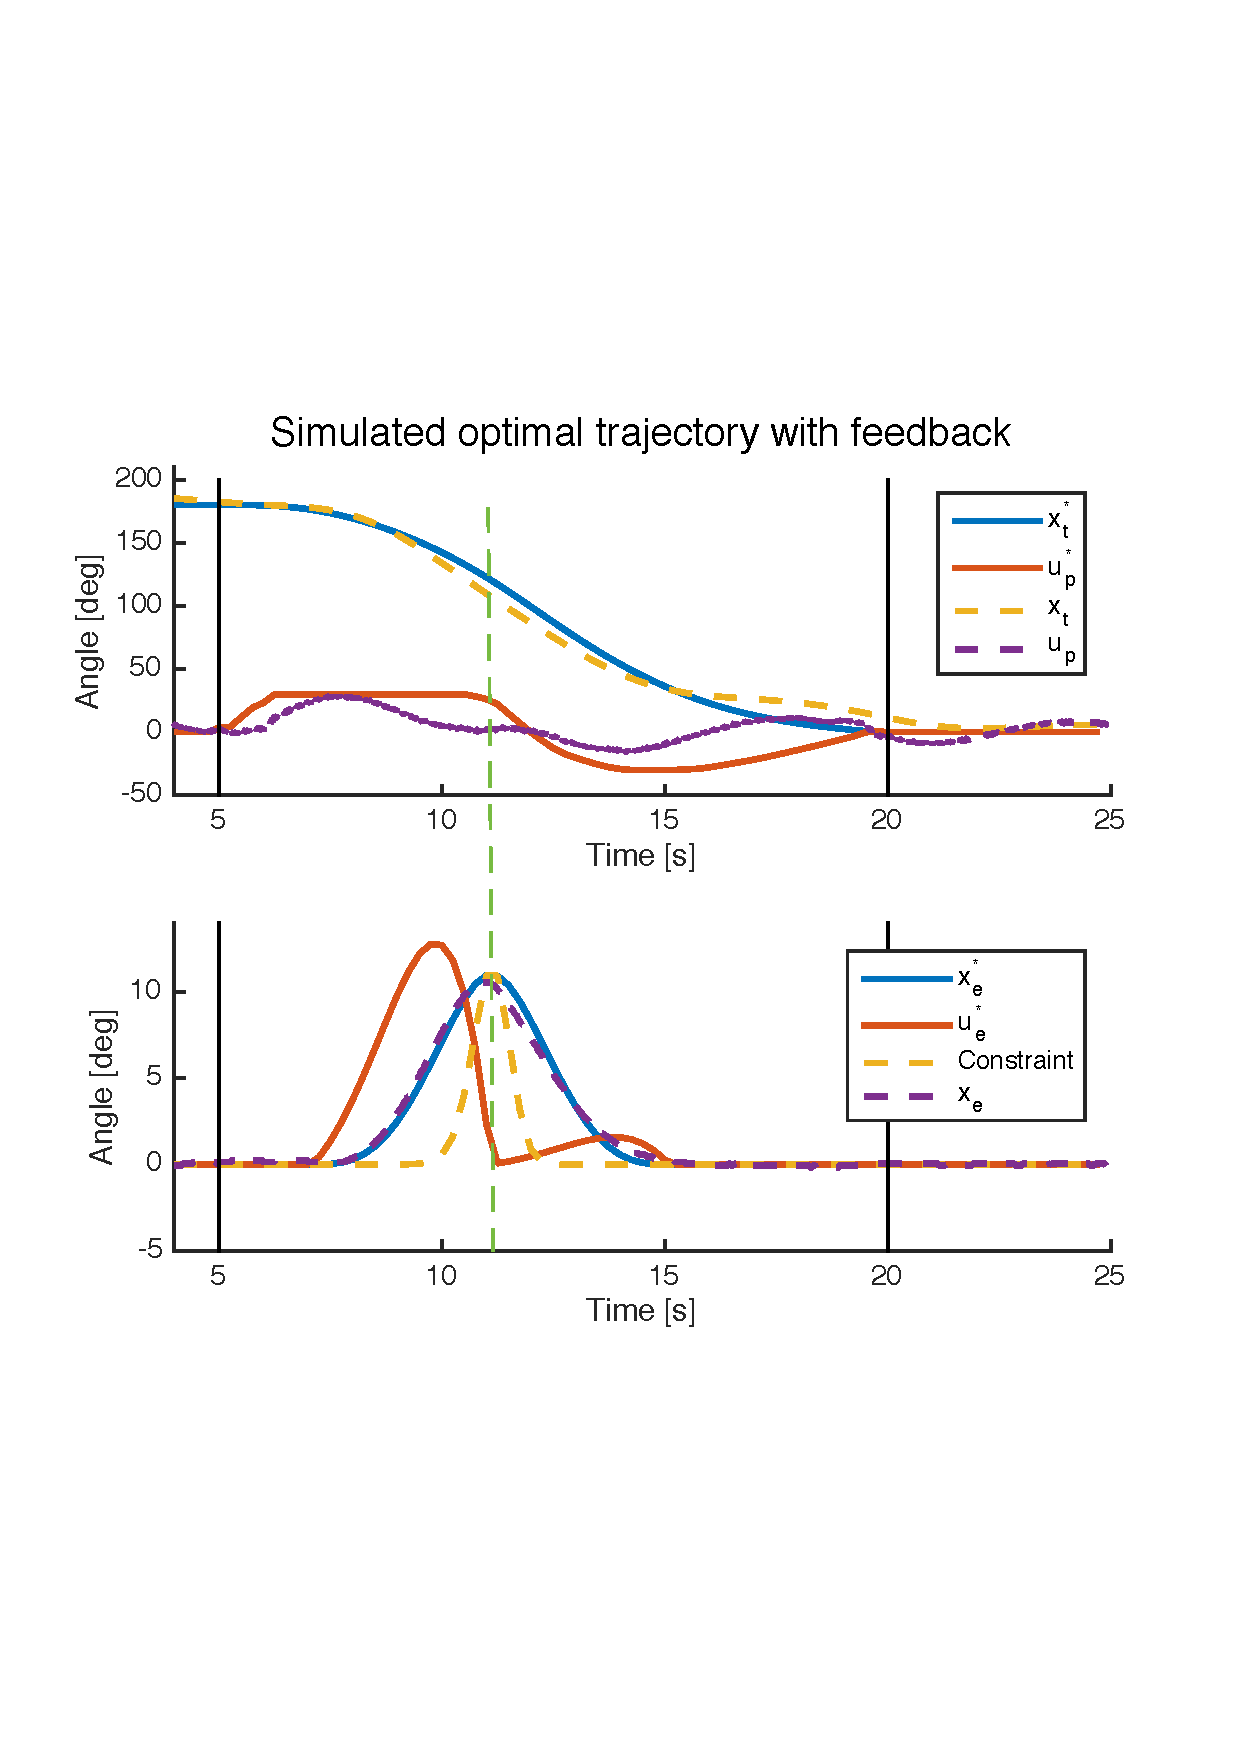
\includegraphics[width=1.2\textwidth]{figures/day4_cl/plot_day4_CL_q_20_1_1_1_20_1_marked2}}
	\caption{Coupling between pitch and elevation}
	\label{fig:coupling_pitch_elev}
\end{figure}

\section{Discussion}\label{sec:discussion}
\subsection{Optimal control without feedback}
When controlling the helicopter with only the estimated optimal input sequence, the deviation due to linearization and modelling errors became too large, and the helicopter deviated drastically from the optimal trajectory. However, there was one benefit from using optimal control without feedback; the ability to limit inputs. So if the system need optimal control with limits on states and inputs, and in addition feedback, MPC is the way to go. See section below.

\subsection{Optimal control with feedback}
While the open-loop optimal control was quite poor, the closed-loop configuration with a LQR was quite promising. Because of modelling errors, the optimal input sequence calculated did not lead to the helicopter following its optimal travel or elevation trajectory, and we ended up with the helicopter drifting away from the solution. Because of this, we had to penalize deviations in these trajectories rather than pitch. Another effect of including feedback on an optimal trajectory was that the final input was no longer guaranteed to be within the constraints of the optimization problem.

\subsection{MPC with implicit feedback}
As mentioned in the first section, the optimal open-loop configuration performed quite poor due to the lack of feedback. This is where MPC makes an entry, with its re-optimization on every time step with the measured/estimated state as initial condition. Only the first step of the input sequence is used. This is because the new measurement on the next step will give a better trajectory. This way you get both implicit feedback and the ability to set constraints on states and inputs. 
\section{Conclusion}\label{sec:conclusion}
Our results and discussion clearly points towards MPC as the most useful way of controlling a plant such as the helicopter model. However, it it also the most expensive algorithm in terms of computational power needed, and therefore might be considered as overkill in many small systems or systems with lower requirements on optimality.
\afterpage{\null\newpage}

\appendix
\section{MATLAB Code}\label{sec:matlab}

\subsection{Day 2}\label{code:day2}
\lstinputlisting{code/day2/day2.m}

\newpage
\subsection{Day 3}\label{code:day3}
\lstinputlisting{code/day3/day3.m}

\newpage
\subsection{Day 4 open-loop}\label{code:day4_ol}
\lstinputlisting{code/day4_openloop/day4_openloop.m}

\newpage
\subsection{Day 4 closed-loop}\label{code:day4_cl}
\lstinputlisting{code/day4/day4.m}
\section{Simulink Diagrams}\label{sec:simulink}
\begin{figure}[ht!]
	\centering
 	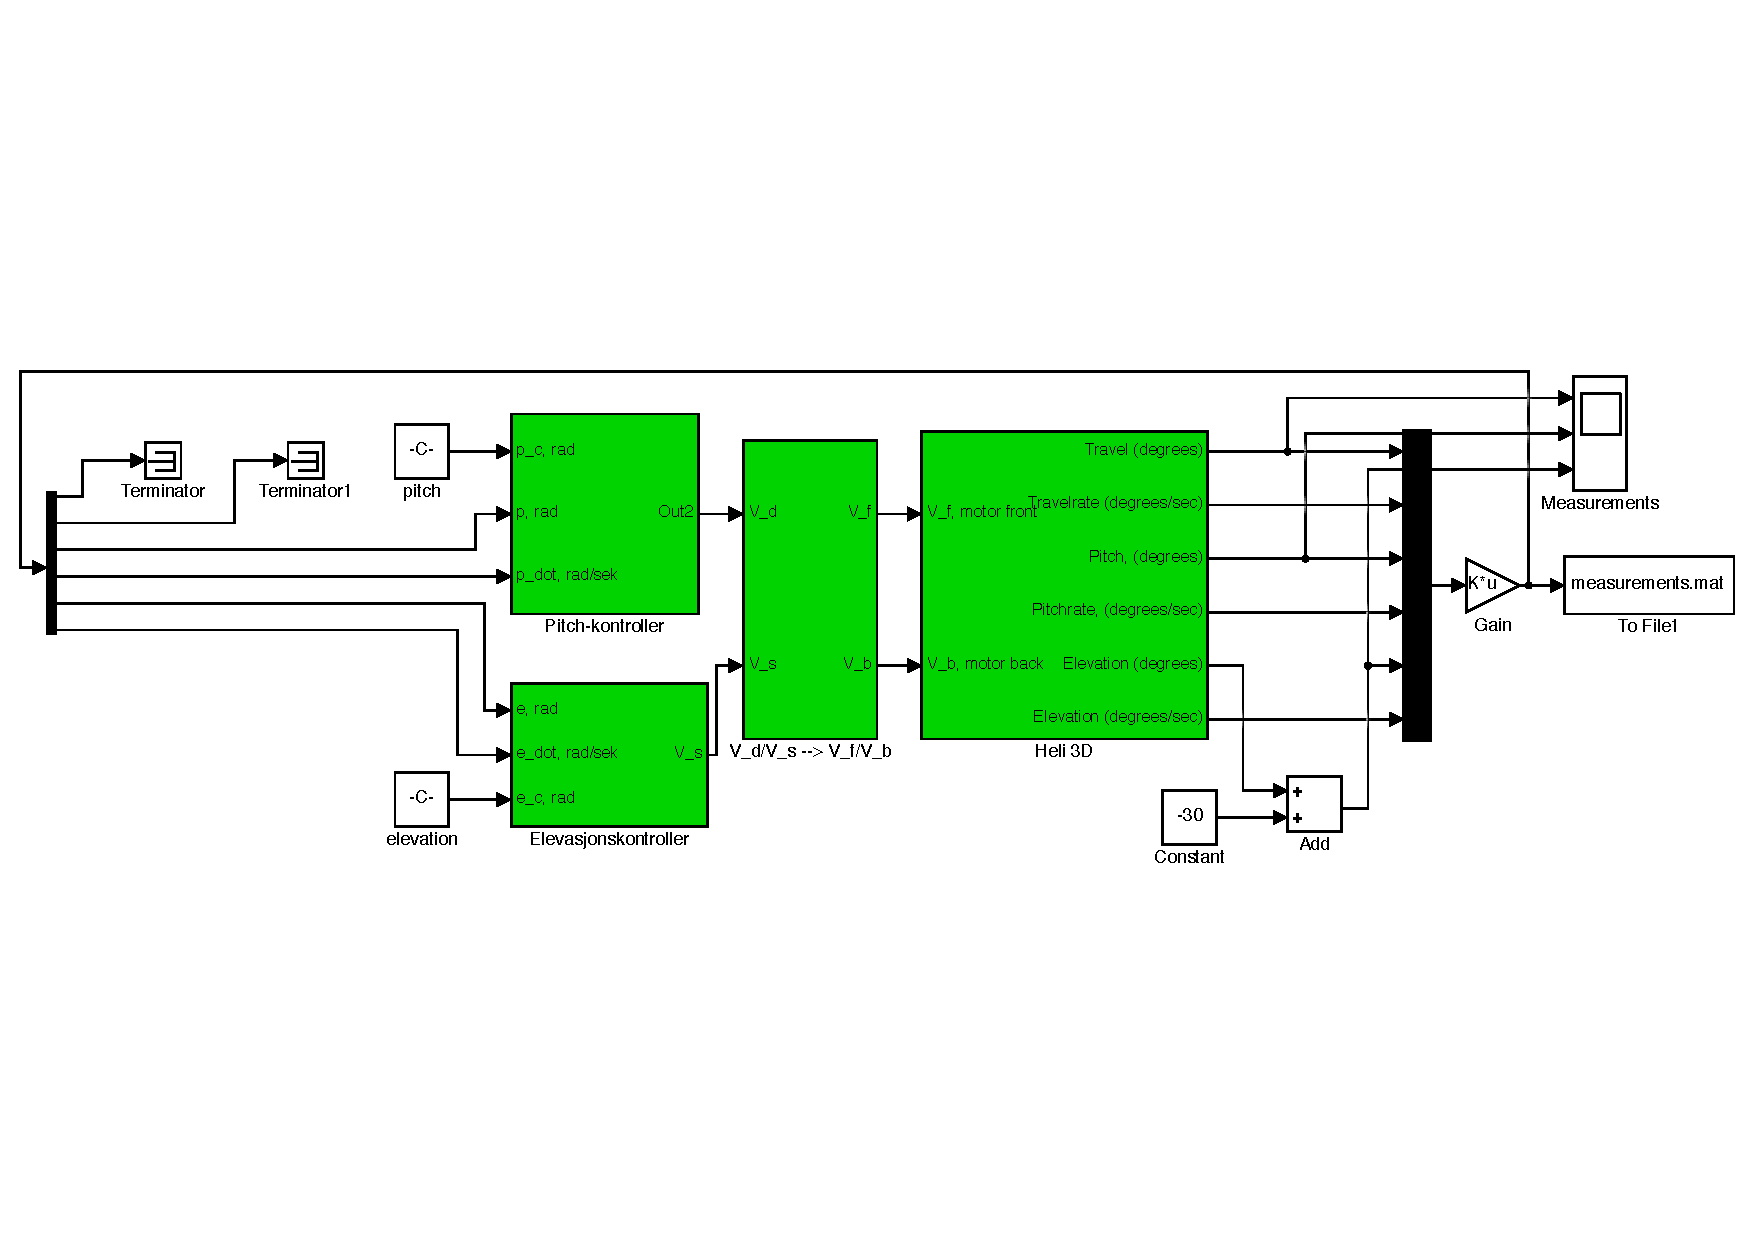
\includegraphics[width = 0.8\textwidth]{figures/day2/day2_mdl}
 	\caption{Simulink optimal open-loop model}
 	\label{fig:simulink_day2}
\end{figure}
\begin{figure}[ht!]
	\centering
 	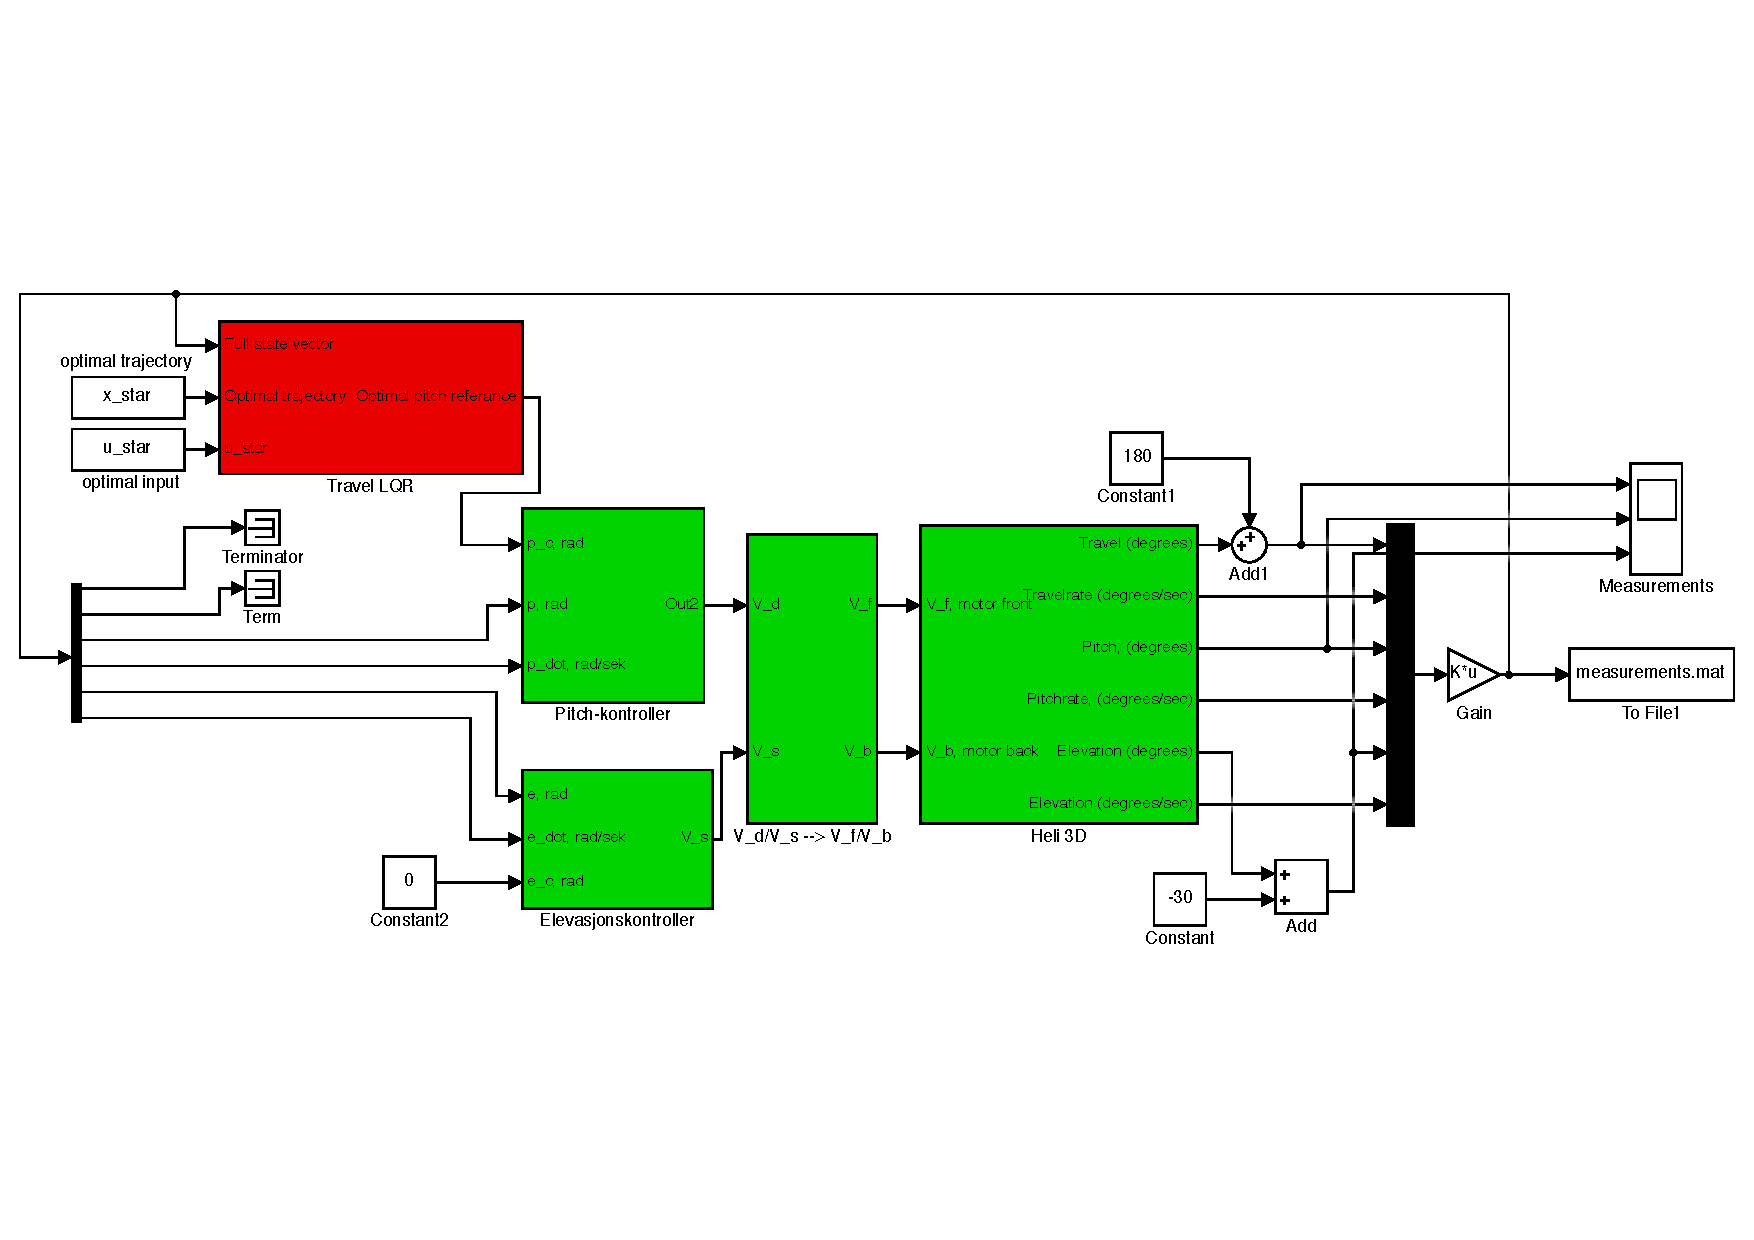
\includegraphics[width = 0.8\textwidth]{figures/day3/day3_mdl}
 	\caption{Simulink optimal closed-loop model}
 	\label{fig:simulink_day3}
\end{figure}
\begin{figure}[ht!]
	\centering
 	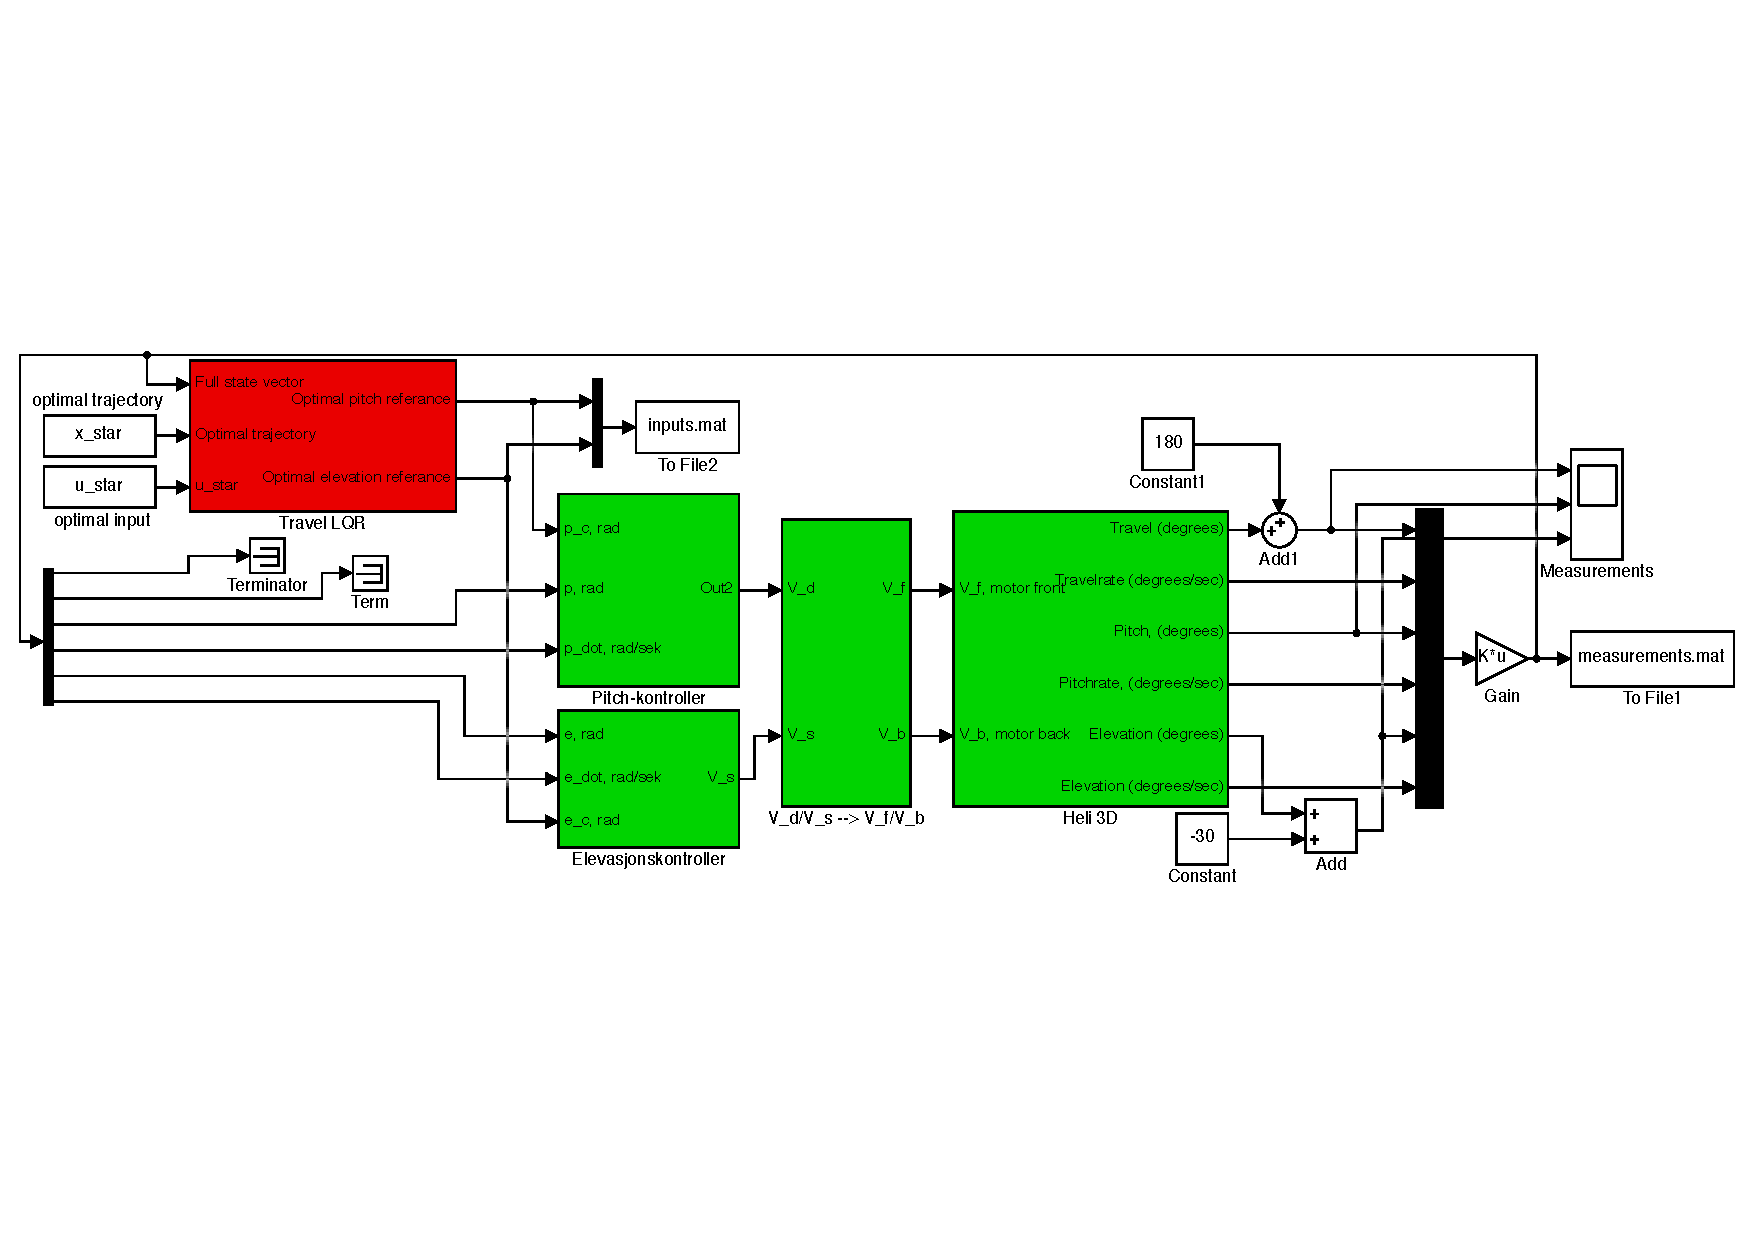
\includegraphics[width = 0.8\textwidth]{figures/day4_cl/day4_cl_mdl}
 	\caption{Simulink optimal closed-loop model in two dimensions}
 	\label{fig:simulink_day4_cl}
\end{figure}
\begin{figure}[ht!]
	\centering
 	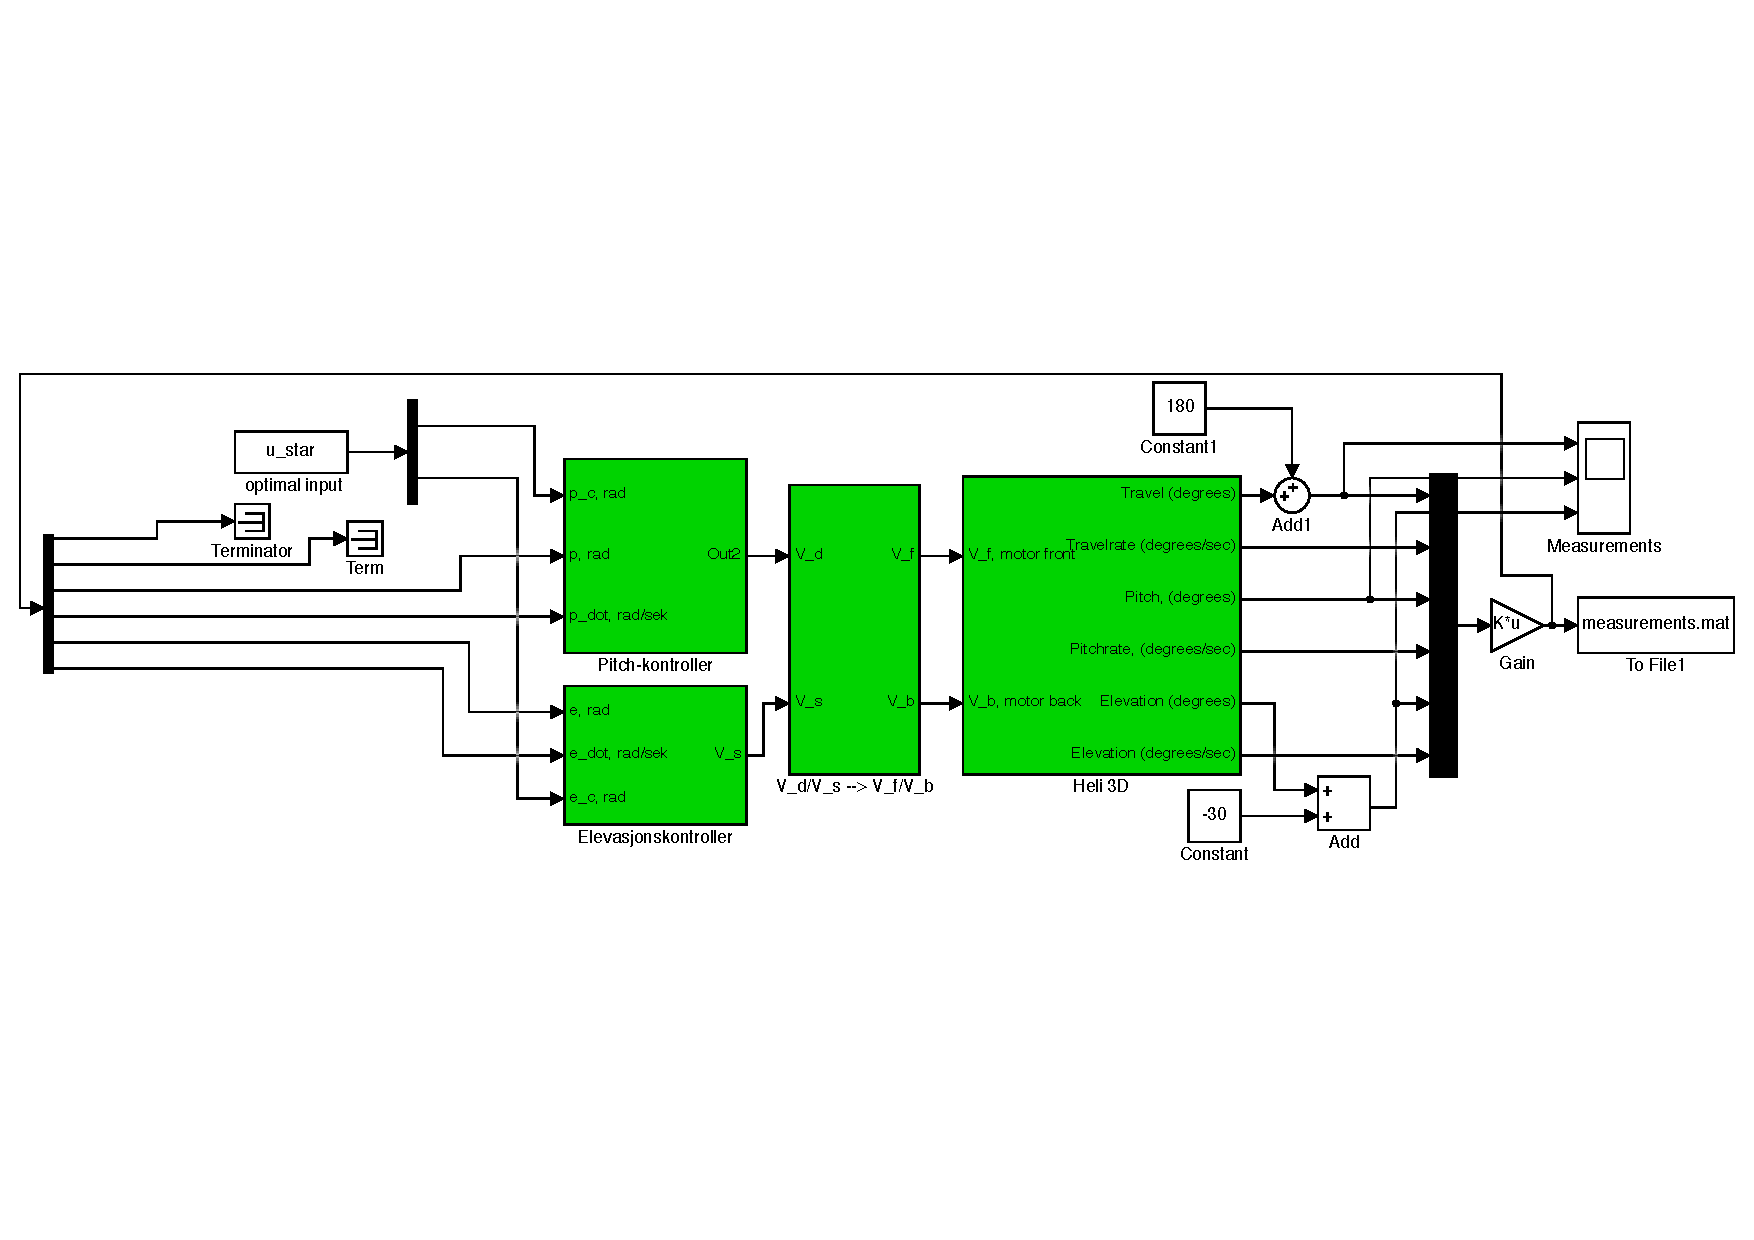
\includegraphics[width = 0.8\textwidth]{figures/day4_ol/day4_ol_mdl}
 	\caption{Simulink optimal open-loop model in two dimensions}
 	\label{fig:simulink_day4_ol}
\end{figure}

\clearpage
\bibliographystyle{apalike}
\bibliography{helibib}\label{sec:bibliography}

\end{document}
